\documentclass{article}
\usepackage{iclr2018_conference, times}
\usepackage{hyperref}       % hyperlinks
\usepackage{url}            % simple URL typesetting
\usepackage{booktabs}       % professional-quality tables
\usepackage{amsfonts}       % blackboard math symbols
\usepackage{nicefrac}       % compact symbols for 1/2, etc.
\usepackage{microtype}      % microtypography
\usepackage{amsmath}
\usepackage{hyperref}
\usepackage{graphicx}

\definecolor{mydarkblue}{rgb}{0,0.08,0.45}
\hypersetup{colorlinks=true,
    linkcolor=mydarkblue,
    citecolor=mydarkblue,
    filecolor=mydarkblue,
    urlcolor=mydarkblue}

\newcommand{\vtheta}{\mathbf{\theta}}
\newcommand{\relaxed}{r}
\newcommand{\controlf}{\hat g}  % Control variate for functions
\newcommand{\controlg}{\hat g}  % Control variate for gradients
\newcommand{\discreteDist}{p(b|\theta)}
\newcommand{\loss}{f(b)}
\newcommand{\lossGrad}{\loss{} \frac{\partial}{\partial \theta }\log \discreteDist{}}
\newcommand{\mcGrad}{\hat{g}}
\newcommand{\expectedLoss}{\mathbb{E}_{\discreteDist{}} \! \left[ \, \loss{} \right]}
\newcommand{\expectedLossLogTrick}{\mathbb{E}_{\discreteDist{}} \! \left[ \, \lossGrad{} \right]}
\newcommand{\var}{\mathbb{V}}
\newcommand{\vu}{\mathbf{u}}
\newcommand{\E}{\mathbb{E}}
\newcommand{\LL}[1]{\frac{\log \pi(a_{#1}| s_{#1}, \theta)}{\partial \theta}}
\newcommand{\PT}{\frac{\partial}{\partial \theta}}
\newcommand{\PP}[1]{\frac{\partial}{\partial #1}}
\newcommand{\PPH}{\frac{\partial}{\partial \phi}}
\newcommand{\LP}[1]{\PT \log p(#1)}
\newcommand{\LZ}[1]{\frac{\log \pi(z_{#1}| s_{#1}, \theta)}{\partial \theta}}



\title{Backpropagating through the Void:\\ Optimizing Differentiable Control Variates}

\author{
  Will S. Grathwohl\thanks{Use footnote for providing further
    information about author (webpage, alternative
    address)---\emph{not} for acknowledging funding agencies.} \\
  University of Toronto\\
  Vector Institute\\
  Toronto, ON \\
  \texttt{wgrathwohl@cs.toronto.edu} \\
}

\begin{document}
\maketitle
\begin{abstract}
Gradient-based optimization is the foundation of deep learning and reinforcement learning.
Even when the mechanism being optimized is unknown or not differentiable, optimization using high-variance or biased gradient estimates is still often the best strategy.
We introduce a general framework for learning low-variance, unbiased gradient estimators for black-box functions of random variables.
These estimators can be jointly trained with model parameters or policies, and are applicable in both discrete and continuous settings.
We give unbiased, adaptive analogs of state-of-the-art reinforcement learning methods such as deep deterministic policy gradients and advantage actor-critic.
We also demonstrate this framework for training discrete latent-variable models.
\end{abstract}


\section{Introduction}
Gradient-based optimization has been key to most recent advances in machine learning and reinforcement learning.
The back-propagation algorithm \citep{rumelhart1986learning}, also known as reverse-mode automatic differentiation~\citep{speelpenning1980compiling, rall1981automatic} computes exact gradients of deterministic, differentiable objective functions.
The reparameterization trick \citep{williams1992simple, kingma2013autoencoding, rezende2014stochastic} allows backpropagation to give unbiased, low-variance estimates of gradients of expectations of continuous random variables.
This has allowed effective stochastic optimization of large probabilistic latent-variable models.

%Unfortunately, backpropagation cannot be easily applied to problems involving discrete random variables, or when the function being optimized is a black box~\citep{schulman2015gradient}.
Unfortunately, there are many objective functions relevant to the machine learning community for which backpropagation cannot be applied. In reinforcement learning, for example, the function being optimized is unknown to the agent and is treated as a black box~\citep{schulman2015gradient}. Similarly, when fitting probabilistic models with discrete latent variables, discrete sampling operations create discontinuities giving the objective function zero gradient with respect to its parameters.
%This is the case in most reinforcement learning settings, or when fitting probabilistic models with discrete latent variables.
Much recent work has been devoted to constructing gradient estimators for these situations.
In reinforcement learning, advantage actor-critic methods~\citep{mnih2016asynchronous} give unbiased gradient estimates with reduced variance obtained by jointly optimizing the policy parameters with an estimate of the value function.
In discrete latent-variable models, low-variance but biased gradient estimates can be given by continuous relaxations of discrete variables~\citep{maddison2016concrete, jang2016categorical}.

A recent advance by \citet{tucker2017rebar} used a continuous relaxation to construct a control variate \cite{paisley} for functions of discrete random variables. Low-variance estimates of the expectation of the control variate can be computed using the reparameterization trick to produce an unbiased estimator with lower variance than previous methods.

Furthermore, \citet{tucker2017rebar} showed how to tune the free parameters of these relaxations to minimize their variance during training.

%\paragraph{Contributions}
In this work we generalize the method of \citet{tucker2017rebar} to learn a free-form control variate parameterized by a neural network, giving a lower-variance, unbiased gradient estimator which can be applied to a wider variety of problems with greater flexibility.
 
Most notably, our method is applicable even when no continuous relaxation is available, as in reinforcement learning or black box function optimization.

Furthermore, we derive improved variants of popular reinforcement learning methods with unbiased gradient estimates, lower variance, and more stable training dynamics.

%\paragraph{Contributions}
%\begin{itemize}
%\item we keep conditional reparam from rebar while exploring and expanding on gradient signal for minimizing variance of estimator
%\item we generalize the concrete and muprop relaxations for a learnable family of functions that can be optimized via gradient decent to minimize the variance of the estimator
%\item We show that concrete relax is not optimal, and that control variate based on the discrete objective at continuous input is is not the optimal control variate.
%\item we combine these insights into a new family of estimators that generalizes rebar
%\end{itemize}

\begin{figure}[h]
\begin{center}
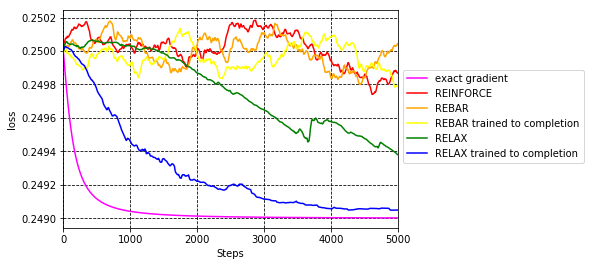
\includegraphics[width=.3\textwidth]{figures/losses}
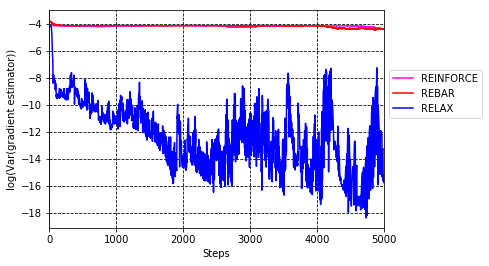
\includegraphics[width=.3\textwidth]{figures/variance_no_opt}
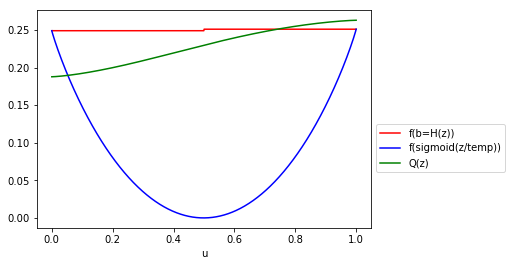
\includegraphics[width=.3\textwidth]{figures/learned_r}
\label{first figure}
\end{center}
\caption{
\emph{Left:} Estimator losses.
\emph{Centre:} Estimator variance.
\emph{Right:}Learned relaxation function.
}
\end{figure}

%\section{Motivation}
%(WE SHOULD BREAK THIS UP INTO MOTIVATION AND BACKGROUND)
%IE 	WHY DO WE WANT THIS, RL, DISCRETE RANDOM VARIABLE MODELS, YADDA, YADDA, YADDA

%THEN HOW HAS IT BEEN DONE IN THE PAST

%THEN WHATS WRONG WITH THAT, LIMITATIONS, SHIT LIKE THAT
%\subsection{optimizing continuous black-box functions}
%\label{continuous}
%Deep deterministic policy gradients \citep{lillicrap2015continuous}

%Also: \citep{levine2016end}

\section{Background: Gradient estimators}


How can we choose the parameters of a distribution to maximize an expectation?
This problem comes up in reinforcement learning, where we must choose the parameters $\theta$ of a policy distribution $\pi(a|s, \theta)$ to maximize the expected reward $\mathbb{E}_{\tau \sim \pi} \left[ R \right]$ over state-action trajectories $\tau$.
It also comes up in fitting latent-variable models, when we wish to maximize the marginal probability ${p(x|\theta) = \sum p(x|z) p(z|\theta) = \mathbb{E}_{p(z|\theta)} \left[ p(x|z) \right]}$.
In this paper, we'll consider the general problem of optimizing
%
\begin{align}
\mathcal{L}(\theta)=\expectedLoss{}.
\end{align}
%
%Later, we will discuss the case when $\loss{}$ depends directly on $\theta$.

When the parameters $\theta$ are high-dimensional, gradient-based optimization is a appealing because it provides information about how to adjust each parameter individually.
Stochastic optimization is essential for large problems, but is only guaranteed to converge to a fixed point of the original objective~\citep{robbins1951stochastic} when the stochastic gradients $\hat g$ are unbiased, i.e. ${\mathbb{E} \left[ \hat g \right] = \PT \mathbb{E}_{p(b|\theta)} \left[ f(b) \right]}$.

Below we review past work in gradient estimation.

\paragraph{The score-function gradient estimator}
One of the most generally-applicable gradient estimators is known as the score-function estimaor, or REINFORCE~\citep{williams1992simple}:
%
\begin{align}
\hat g_\textnormal{reinforce} =  f \left( b \right) \PT \log p(b | \theta), \qquad b \sim p(b | \theta)
\end{align}
%
This estimator is unbiased, but in general has high variance.
Intuitively, this estimator is limited by the fact that it doesn't use any information about how $f$ depends on $b$, only on the final outcome of evaluating $f(b)$.

\paragraph{The reparameterization trick}
When $f$ is continuous and differentiable, and the latent variables $b$ can be written as a deterministic, differentiable function of a random draw from a fixed distribution, the reparameterization trick \citep{williams1992simple, kingma2013autoencoding, rezende2014stochastic} creates a low-variance, unbiased gradient estimator by making the dependence of $b$ on $\theta$ explicit:
%
\begin{align}
%\hat g_\textnormal{reparam} = \frac{\partial f \left( b(\theta, \epsilon) \right)}{\partial \theta}, \qquad \epsilon \sim p(\epsilon)
\hat g_\textnormal{reparam} = \PT f \left( b(\theta, \epsilon) \right), \qquad \epsilon \sim p(\epsilon)
\end{align}
%
This gradient estimator is often used when training high-dimensional, continuous latent-variable models, such as variational autoencoders or GANs.
One intuition for why this gradient estimator is preferable to REINFORCE is that it depends on $\partial f / \partial b$, which directly exposes the dependence of $f$ on $b$.

\paragraph{Concrete relaxation}
When $b$ is discrete and $f$ is known, one general approach is to differentiate a continuous relaxation of the discrete random variables.
\cite{maddison2016concrete} and \cite{jang2016categorical} developed a differentiable relaxation of the categorical distribution, called the concrete distribution:
%
\begin{align}
\hat g_\textnormal{concrete} = \PT f \left( \sigma_\lambda ( \log \theta - \log(-\log u)) \right), \qquad u \sim \textnormal{uniform}[0, 1] 
\end{align}
%
where $\sigma_\lambda$ is the softmax function with temperature $\lambda$. A similar relaxation for the Bernoulli distribution has been developed as well (see Appendix for details)
This gradient estimator is fairly effective in practice, but produces biased gradients, hindering its usage.
Additionally, it is not clear how to set the temperature $\lambda$ and it is often treated as a hyperparameter.

\paragraph{Control variates}
Control variates are a general method for reducing the variance of a Monte Carlo estimator.
Given an estimator $g(b)$, a control variate is a function $\controlf(b)$ with a known mean $\mathbb{E}_{p(b)} [ \controlf ]$.
Subtracting the control variate from our estimator and adding its mean gives us a new estimator:
%
\begin{align}
\hat g_\textnormal{new}(b) = g(b) - \controlf(b) + \mathbb{E}_{p(b)}[\controlf(b)]
\end{align}
%
This new estimator has the same expectation as the old one:
%
\begin{align}
\mathbb{E}_{p(b)}\left[ g_\textnormal{new}(b) \right] 
= \mathbb{E}_{p(b)}\left[g(b) - \controlf(b) + \mathbb{E}_{p(b)} \left[ \controlf(b) \right] \right]
%= \mathbb{E}_{p(b)}\left[f(b) \right] - \mathbb{E}_{p(b)} \left[ \controlf(b) \right] + \mathbb{E}_{p(b)} \left[ \controlf(b) \right]
= \mathbb{E}_{p(b)}\left[ g(b) \right]
\end{align}
%
Importantly, the new estimator has lower variance than $g(b)$ if $\controlf(b)$ is positively correlated with $f(b)$.

\paragraph{REBAR}
The recently-developed REBAR method \citep{tucker2017rebar} estimates the gradient of expectations of functions of Bernoulli random variables. This method uses the REINFORCE estimator with a control variate. The control variate is derived from the original loss function evaluated at continuously-relaxed inputs \citep{maddison2016concrete, jang2016categorical}. The expectation of this control variate is estimated with low variance via the reparameterization trick. 

The authors restrict their analysis to the case wehre $p(b|\theta) = \text{Bern}(b|\theta)$. Samples are drawn from $p(b|\theta)$ with a determanistic function of a continuous, reparameterizable random variable $z$. 
\begin{align}
z &:= g(u, \theta) = \log\frac{\theta}{1-\theta} + \log\frac{u}{1-u}, \qquad u \sim \text{uniform}[0,1]\nonumber\\
b &:= \mathbb{I}(z>0)\nonumber
\end{align}
Thus, we can think of $p(b|\theta)$ as $\int p(b|z, \theta)p(z|\theta)dz$. The REBAR estimator is derived from this realization, noting:
\begin{align}
\PT \expectedLoss{} &= \PT \E_{p(b|\theta)}\left[ f(b) \right] - \E_{p(z|\theta)}\left[ f(\sigma_\lambda(z) \right] + \E_{p(z|\theta)}\left[ f(\sigma_\lambda(z) \right]\nonumber\\
&= \PT \E_{p(b|\theta)}\left[ f(b) - \E_{p(z|b, \theta)}\left[ f(\sigma_\lambda(z) \right]  \right] + \E_{p(z|\theta)}\left[ f(\sigma_\lambda(z) \right]\nonumber\\
&= \E_{p(b|\theta)}\left[\left( f(b) - \E_{p(z|b, \theta)}\left[ f(\sigma_\lambda(z) \right] \right)\PT \log p(b|\theta)  - \PT \E_{p(z|b, \theta)}\left[ f(\sigma_\lambda(z) \right] \right]\nonumber\\
&\qquad + \E_{p(z|\theta)}\left[ f(\sigma_\lambda(z) \right]\nonumber
\end{align}
where $\sigma_\lambda$ is the sigmoid function with temperature $\lambda$. The REBAR estimator is the single-sample monte-carlo estimator derived from the last line above. The REBAR estimator is computed as:
\begin{align}
\hat g_\textnormal{REBAR} = \left(f(b) - f(\sigma_\lambda(z)\right)\PT \log p(b|\theta) + \PT f(\sigma_\lambda(z)) - \PT f(\sigma_\lambda(\tilde{z}))\nonumber\\
z \sim p(z|\theta), \tilde{z} \sim p(z|b, \theta), b = \mathbb{I}(z>0)\nonumber
\end{align}
Details of how to sample from $p(z|b, \theta)$ as well as an extension to categorical random variables can be found in the Appendix. \cite{tucker2017rebar} also introduced a way to optimize the temperature parameter $\lambda$ via gradient decent to minimize the variance of the estimator. 



%\subsubsection{Reducing gradient variance through control variates}
%The core of the REBAR estimator is a REINFORCE-style estimate of a non-differentiable reparameterization of the discrete latent variable as $b=H(z)$, where $H$ is the hard-threshold function an
%\begin{align}
%z := g(u, \theta) := \log\frac{\theta}{1-\theta} + \log\frac{u}{1-u}, u \sim \text{Unif}[0,1]
%\end{align}
%While $z$ is a reparameterization that renders the parameters of $b$ learnable by gradient-based methods, $H$ introduces a new discontinuity in the loss.
%Instead of relaxing the hard threshold as in \cite{maddison2016concrete}, \cite{tucker2017rebar} uses a REINFORCE estimator for the gradient reparameterized with $H(z)$:
%\begin{align}
%    \frac{\partial}{\partial \theta} \mathbb{E}_{p(b)}[f(b)] = \frac{\partial}{\partial \theta} \mathbb{E}_{p(u)}[f(H(z))] = \mathbb{E}_{p(u)}[f(H(z))\frac{\partial}{\partial \theta}\log p(z)]
%\end{align}
%This allows the parameters $\theta$ to be learned using gradient information, but the loss is still non-differentiable due to the hard threshold.
%Since this uses a REINFORCE estimator, it also has high variance.

%Hence, \cite{tucker2017rebar} develop a control variate. A natural continuous relaxation of the hard threshold function is the sigmoid function, leading \cite{tucker2017rebar} to choose a $H(z) \approx \sigma_\lambda(z) := \sigma(z / \lambda) = (1+\exp( - z / \lambda))^{-1}$.
%This relaxation leads to the following control variate summed with its expectation:
%\begin{align}
%    \frac{\partial}{\partial \theta} \mathbb{E}_{p(z)}[f(\sigma_\lambda(z))] =  \mathbb{E}_{p(z)}[f(\sigma_\lambda(z))\frac{\partial}{\partial \theta}\log p(z)].
%\end{align}
%Unfortunately, simply applying this control variate was found to be ineffective. 
%The author's key insight was to derive a low-variance form of this control variate that takes advantage of a conditional marginalization of the reparameterized $z$ given a particular choice of discrete $b$.
%This introduces a second reparameterization $\tilde{z}$ of $p(z|b)$, which depends on another sample $v\sim \text{Unif}[0,1]$.
%See \cite{tucker2017rebar} for details of the derivation.


%The control variate has the following form:
%\begin{align}
%    f(\sigma_\lambda(\tilde{z}))\frac{\partial}{\partial \theta}\log p(H(z))
%\end{align}
%and noting that 
%\begin{align}  \mathbb{E}_{p(u,v)}[f(\sigma_\lambda(\tilde{z}))\frac{\partial}{\partial \theta}\log p(H(z))] = \mathbb{E}_{p(u,v)}[\frac{\partial}{\partial \theta}f(\sigma_\lambda(\tilde{z}))  - \frac{\partial}{\partial \theta} f(\sigma_\lambda(z))]
%\end{align}
%gives us the REBAR gradient estimator: \begin{align}
%    \frac{\partial}{\partial \theta} \mathbb{E}_{p(b)}[f(b)] = \mathbb{E}_{p(u,v)}[f(\sigma_\lambda(\tilde{z}))\frac{\partial}{\partial \theta}\log p(H(z))  - \eta f(\sigma_\lambda(\tilde{z}))\frac{\partial}{\partial \theta}\log p(H(z)) + \eta\frac{\partial}{\partial \theta} f(\sigma_\lambda(z)) - \eta\frac{\partial}{\partial \theta}f(\sigma_\lambda(\tilde{z})) ]
%\end{align} where $\eta$ is trained to minimize the variance of the estimator. 

% ** TODO: place \eta in this equation?
%The special form of $\tilde{z}$ yields a lower-variance gradient estimate because a number of the random variables are conditionally marginalized out of the estimator.
%Two features of this control variate make it particularly effective: its high correlation with the REINFORCE gradient, and a low-variance, reparameterized form of certain terms in the estimator.

\section{Scope and Limitations}
\label{limitations}
While the above approaches have greatly broadened the scope of functions whose derivatives we can approximate, there still exist a number of factors limiting their application to many problems of interest.

The bias induced by the concrete relaxation can lead to convergence at unsuitable optima or no convergence at all. REBAR alleviates these issues by using the relaxation as a control variate for the estimator instead of the estimator itself. Unfortunately, REBAR requires the function being optimized, whose input is only defined at discrete inputs, to also accept continuous inputs, be differentiable w.r.t. those inputs, and behave predictably with respect to those continuous inputs. While often true, these are strong assumptions to make. Furthermore, REBAR and the concrete relaxation require that the function being optimized is known. 

This makes REBAR and the concrete relaxation inapplicable for optimizing black-box functions, as in reinforcement learning settings where the reward is an unknown function of the environment.


\section{A General Family of Gradient Estimators}
In this work, we seek to synthesize and generalize the approaches introduced above. Mainly, we desire a simple and generic gradient estimator that can be applied to expectations of known or black-box functions of discrete or random variables. We would like these approaches to be simple to implement and add minimal computational overhead. 

The foundation of our approach is the score function gradient estimator with a control variate who's expectation can be estimated with low variance using the reparameterization trick. This control variate is neural network which is trained directly to minimize the variance of the estimated gradients. The central result of this paper is that learning the function in the control variate leads to even better convergence properties and lower variance gradient estimates. 

We first outline the algorithm when we are optimizing $E_{p_\theta(b)}[f(b)]$ where $b$ is a continuous random variable and then when $b$ is discrete.

\subsection{Continuous Variables}
We wish to compute $\PT\E_{p_\theta(b)}[f(b)]$ where $p_\theta(b)$ is a distribution with continuous support that admits a reparameterization $T$ such that $T(\theta, \epsilon) = b \sim p_\theta(b)$ where $\epsilon \sim p(\epsilon)$. We assume that $f$ is a black-box or involves operations such that $\PT f = 0$ almost everywhere or is not computable.  Given the reparameerization, we can re-write this as an expectation over $\epsilon$ as  $\PT\E_{p(\epsilon)}[f(T(\epsilon, \theta)]$. We introduce a new, differentiable function $r_\phi$ and define our estimator below.

\begin{align}
\PT\E_{p_\theta(b)}[f(b)] \approx g_\phi(\epsilon) &= \Big[f(b) - r_\phi(b)\Big]\cdot\LP{b} + \PT r(b)\\
&= \Big[f(T(\epsilon, \theta)) - r_\phi(T(\epsilon, \theta))\Big]\cdot\LP{b} + \PT r(T(\epsilon, \theta))
\end{align}

We note that our estimator is unbiased for all choices of $r_\phi$, i.e $\E_\epsilon[g_\phi(\epsilon)] = \PT\E_{p_\theta(b)}[f(b)]$. A proof can be found in the appendix. 

\subsection{Discrete Variables}
In the case where $p_\theta(b)$ is a distribution over discrete variables, we introduce some notation. We assume there exist a continuous distribution $p_\theta(z)$ and a determanistic mapping $H$ such that $H(z) = b \sim p_\theta(b)$. If $p(b)$ is Bernoulli then $p_\theta(z) = \text{Logistic}(z|\theta)$ and $H(z) = \mathbb{I}(z>0)$. If $b$ is Categorical, then $p_\theta(z) = \text{Softmax}(z|\theta)$. We also assume that $p_\theta(z)$ is reparameterizable. Moreover, we assume the distribution $p_\theta(z|b)$ is also reparameterizable meaning there exists $\hat{T}$ such that $\hat{T}(\hat{\epsilon}, b, \theta) = \hat{z} \sim p_\theta(\hat{z}|b)$ (see Appendix for details).  

The estimator is based on a 2-step monte-carlo procedure. First we sample $\epsilon \sim p(\epsilon)$ from which we produce $z = T(\theta, \epsilon)$ and $b = H(z)$. We then sample $\hat{\epsilon} \sim p(\hat{\epsilon})$ and produce $\hat{z} = \hat{T}(\hat{\epsilon}, b, \theta)$. We use these values to produce our estimator below.

\begin{align}
\PT\E_{p_\theta(b)}[f(b)] \approx g_\phi(\epsilon,\hat{\epsilon}) &= \Big[f(b) - r_\phi(\hat{z})\Big]\cdot\LP{b} + \PT r(z) - \PT r(\hat{z})\\
&= \Big[f(H(T(\epsilon, \theta))) - r_\phi(\hat{T}(\epsilon, H(T(\epsilon, \theta)), \theta))\Big]\cdot\LP{b}\\ 
&+ \PT r(T(\epsilon, \theta)) - \PT r_\phi(\hat{T}(\epsilon, H(T(\epsilon, \theta)), \theta))
\end{align}

This estimator is also unbiased i.e $E_{\epsilon, \hat{\epsilon}}[g_\phi(\epsilon, \hat{\epsilon})] = \PT\E_{p_\theta(b)}[f(b)]$.

\subsection{Optimizing The Control Variate}
For both estimators, we would like to optimize the parameters $\phi$ to produce the lowest variance. Following \cite{tucker2017rebar}, we note that for any unbiased estimator $g_\phi$ we have 
\begin{align}
\PPH \text{Var}(g_\phi) = \PPH \E[g_\phi^2] - \PPH \E[g_\phi]^2
= \PPH \E[g_\phi^2] - \PPH \E_{p_\theta(b)}[f(b)]
= \PPH \E[g_\phi^2] = \E \left[ \PPH g_\phi^2 \right].
\end{align}

Therefore, we can minimize the variance of the estimator by training to minimize the square of the gradients it produces.
[TODO: talk about how this is probably better than minimizing the squared prediction error]


%The REBAR estimator uses a control variate that evaluates the original loss function at relaxed inputs, reparameterized both unconditionally (denoted $z$, and conditionally, denoted $\tilde{z}$).
%The central result of this paper is that learning the function in the control variate leads to even better convergence properties.
%Specifically, we generalize the conditional marginalization and control variate of REBAR to the following form:
%\begin{align}
%    \mathbb{E}_{p(u,v)}[\relaxed (\tilde{z};\phi)\frac{\partial}{\partial \theta}\log p(H(z))] = \mathbb{E}_{p(u,v)}[\frac{\partial}{\partial \theta} \relaxed(\tilde{z};\phi) - \frac{\partial}{\partial \theta} \relaxed(z; \phi)],
%\end{align}
%where \relaxed{} is a neural network with parameters $\phi$.

%The generalized REBAR estimator replaces the loss function evaluations in the control variate with an adaptive $\relaxed$ function which is trained via gradient decent to minimize the variance of the estimator. As shown in \cite{tucker2017rebar}, this can be easily computed. Denoting the RELAX estimator as $r(\phi)$ we obtain:
%\begin{align}
%  \frac{\partial}{\partial\phi}\var{(r(\phi))} = \frac{\partial}{\partial\phi}\mathbb{E}[r(\phi)^2] + \frac{\partial}{\partial\phi}\mathbb{E}[r(\phi)]^2 = \frac{\partial}{\partial\phi}\mathbb{E}[r(\phi)^2] = \mathbb{E}[\frac{\partial}{\partial\phi}r(\phi)^2]
%\end{align}
%Where the second equality comes from the fact that for all $\phi$, the RELAX estimator is unbiased and therefore $\frac{\partial}{\partial\phi}\mathbb{E}[r(\phi)]^2 = 0$.


%\section{Properties of Optimal Relaxations}
%In \cite{tucker2017rebar} the concrete distribution \cite{maddison2016concrete} is used in the control variate due to its similarity to the Bernoulli distribution.

%NEXT: PROVE THAT CONCRETE IS NOT THE OPTIMAL RELAXATION TO USE (SHOULD BE EASY TO PROVE BUT WE NEED TO DO IT)


%Using variational calculus, we can examine the form of the optimal relaxation $\relaxed{}$

%Relaxing Assumptions

%identifying assumptions other estimators in the past made

%demonstrate (proof?) that those assumptions are not optimal

%and that the optimum is a function of {f, theta}


\section{Applications}
\label{Applications}
We demonstrate the effectiveness of our estimator on a number of challenging optimization problems. Following \cite{tucker2017rebar} we begin with a simple toy example to illuminate the potential of our method and then continue to the more relevant problems of optimize binary VAE's and reinforcement learning.

\subsection{Toy Experiment}
We seek to minimize $\mathbb{E}_{p(b|\theta)}[(b - t)^2]$ as a function of the parameter $\theta$ where $p(b|\theta) = \mathtt{Bern}(b|\theta)$. \cite{tucker2017rebar} set the target $t = .45$.
We focus on the more challenging case where $t = .499$.
With this setting of the target, REBAR and competing methods suffer from high variance and are unable to discover the optimal solution $\theta = 0$.

The fixed Concrete relaxation of REBAR is unable to produce a gradient whose signal outweighs the sample noise and is therefore unable to solve this problem noticeably faster than REINFORCE.
Figure \ref{fig:toy_var} plots the learned relaxations for a fixed value of $\theta$.

It can be seen that RELAX learns a relaxation whose derivative points in the direction of decreased loss for all values of reparameterization noise $u$, whereas REBAR's fixed relaxation only does so for values of $u > t$.


\subsection{Discrete Variational Autoencoder}
As in \citep{tucker2017rebar}, we benchmark the RELAX estimator on the task of training a variational autoencoder \citep{kingma2013autoencoding, rezende2014stochastic} where all random variables are Bernoulli taking values in $\{-1, 1\}$.
As in \cite{tucker2017rebar}, we compare training the variational lower-bound across the MNIST and Omniglot~\citep{lake2015human} datasets.
As in \cite{tucker2017rebar} we test models with 1 and 2 of Bernoulli random variables with linear mappings between them and a model with 1 layer of Bernoulli random variables with non-linear mappings between layers.

We found that due to the complicated structure of the loss function, the RELAX estimator performed worse than REBAR. Instead we add a learned relaxation to REBAR's control variate which we denote relaxed-REBAR.
Our estimator takes the form of \eqref{eq:RELAX} with $$\bar \relaxed(z) = \relaxed(z) + f(\sigma_\lambda(z))$$ where $\relaxed(z)$ is a learned neural network and $f(\sigma_\lambda(z))$ is the Concrete relaxation of REBAR with temperature parameter $\lambda$.
In all experiments, adding the learned $\relaxed(z)$ reduced the variance of the gradients and improved the final results. 

\begin{table}[h]
\begin{center}
\begin{tabular}{l c c c c c} 
& NVIL & MuProp & REBAR & REBAR & RELAX \\
\textbf{MNIST} & & & \citet{tucker2017rebar} & ours & \\\midrule
Nonlinear      & $-102.2$ & $-101.5$ & -101.1  &  -83.02 &  \textbf{-79.49} \\
Linear 1 layer  & $-112.5$ & $-111.7$ & -111.6 & -111.66 & \textbf{-111.22} \\ 
Linear 2 Layer  & $-99.6$ & $-99.07$ & -98.8  & -98.23 & \textbf{-98.04} \\\\
\textbf{Omniglot}\\ \midrule
Nonlinear      & $-110.4$  & $-109.58$ & -108.72  & -62.28 & \textbf{-58.55} \\
Linear 1 layer & $-117.44$ & $-117.09$ & -116.83  & -116.75 & \textbf{-116.62} \\ 
Linear 2 Layer & $-109.98$ & $-109.55$ & -108.99  & -108.74 & \textbf{-108.59}
\end{tabular}
\end{center}
\label{tab:vae}
\caption{Training variational lower bound after training.}
\end{table}

In \citep{tucker2017rebar}, a separate REBAR estimator was used to estimate the gradients of each model parameter (each weight matrix and bias vector).
To apply our estimator to this formulation, we would need to learn a separate relaxation for each model parameter.
To get around this, we use our gradient estimator to approximate $g_\phi \approx \PT \E_{q(b|\theta)}[f(b)]$ where $x\cdot W = \theta$ is the parameters of the Bernouli latent variables, $W$ is our layer's weight matrix. We then obtain an estimate of $\PP{W} \E_{q(b|\theta)}[f(b)] = g_\phi\cdot \frac{\partial \theta}{\partial W}$. We note this gives us unbiased gradients because 
\begin{align}
\E_\epsilon[g_\phi(\epsilon) \cdot \frac{\partial \theta}{\partial W}] = \E_\epsilon[g_\phi(\epsilon)] \cdot \frac{\partial \theta}{\partial W} =  \PT \E_{q(b|\theta)}[f(b)] \cdot \frac{\partial \theta}{\partial W} = 
\frac{\partial}{\partial W} \E_{q(b|\theta)}[f(b)]
\end{align} 

To provide a fair comparison, we re-implemented REBAR in this way (denoted REBAR-ours in table \ref{tab:vae}).
We believe this explains the large difference in performance between our implementation and that of \citep{tucker2017rebar} for the nonlinear models since there are 3 layers of parameters that all share the same gradient estimator.
In the linear models, each layer has its own gradient estimator making our implementation closer to that of \citep{tucker2017rebar}.



\subsection{Reinforcement Learning}
Reinforcement learning is strong motivating problem for methods similar to ours. In reinforcement learning we seek to optimize the paremters of a policy distribution $\pi(a|s;\phi)$ to maximize the (often discounted) sum of future rewards given that policy $\mathbb{E}_{\pi(\phi)}[\sum_{t=1}^{\infty} r_t]$. We can view the sum of future rewards as a black-box function of our policy's actions $f(a)$. Thus, as before we have reduced the problem to that of estimating $\frac{\partial \mathbb{E}_{\pi(a|\phi)}[f(a)]}{\partial \phi}$ which is the standard policy gradient algorithm \cite{POLICY GRADIENT}. 

We test our approach on simple reinforcement learning environments with discrete actions. We use the RELAX estimator and compare with the advantage actor critic algorithm (A2C \cite{A2C}) as a baseline. In all experiments we utilized the same learning rate for the policy network for RELAX and A2C to so differences in performance depended solely on the control variate used. 

To compare these approaches in the most illustrative setting possible we run these algorithms on one environment at a time, running each episode to completion. After completion, we generate the discounted reward for each timestep, treat the episode as a single batch of data, and perform one step of gradient decent. We test our alrgorithm on the Cart-Pole and Lunar-Lander environments from the OpenAI Gym \cite{gym}. We run the Cart-Pole and Lunar-Lander environments for 250 and 1000 episodes, respectively and plot reward and the log-variance of the policy gradients in figure X.

\subsection{RL Introduction}
We seek to compute $$\frac{\partial \E_\tau[R]}{\partial \theta} = \E\Big[\sum_{t=1}^T \LL{t} \sum_{t'=t}^T r_t\Big]$$ but the estimator on the right hand side can have potentially high variance. Instead, we typically compute $$\frac{\partial \E_\tau[R]}{\partial \theta} = \E_\tau\Big[\sum_{t=1}^T \LL{t} [(\sum_{t'=t}^T r_{t'}) - b(s_t)]\Big]$$

This is unbiased because
\begin{align}
\\E_{a_{1:T},s_{1:T}}\Big[\LL{t}\cdot b(s_t)\Big] &= E_{a_{1:t-1},s_{1:t}}\Big[ E_{a_{t:T},s_{t+1:T}} \Big[\LL{t}\cdot b(s_t)\Big]\Big]\\
&= E_{a_{1:t-1},s_{1:t}}\Big[b(s_t)\cdot E_{a_{t:T},s_{t+1:T}} \Big[\LL{t}\Big]\Big]\\
&= E_{a_{1:t-1},s_{1:t}}\Big[b(s_t)\cdot \frac{\partial}{\partial \theta} E_{a_{t:T},s_{t+1:T}} [1]\Big]\\
&= 0
\end{align}

Where $b(s_t)$ is trained to minimize $(b(s_t) - \sum_{i=t}^T r_t)^2.$ This is unbiased for any choice of $b$ since $b$ does not depend on $a_t$. 

\subsubsection{Variance Reduction with RELAX}
We begin the in the case where actions are continuous and any expectation over an action is replaced with an expectation over reparameterization variables $\epsilon$ $$\E_a[f(a)] = \E_\epsilon[f(a(\epsilon))]$$.  We are interested in replacing $b(s_t)$ with a function $m(a_t, s_t)$ which is a function of both actions and states.

This changes the first equation to $$\frac{\partial \E_\tau[R]}{\partial \theta} = \E_\tau\Big[\sum_{t=1}^T \LL{t} [(\sum_{t'=t}^T r_{t'}) - m(a_t, s_t)]\Big]$$ but this makes the estimator biased as $\E_\tau [\LL{t}m(a_t, s_t)] \neq 0$. Because of the dependence on $a_t$ we cannot pull this out of the expectation as we could in line 2 of the above equation.

Instead we subtract out a term who's expectation should be the same as the score function version of the control variate changing our estimator to  $$\frac{\partial \E_\tau[R]}{\partial \theta} = \E_\tau\Big[\sum_{t=1}^T \LL{t} [(\sum_{t'=t}^T r_{t'}) - m(a_t, s_t)] + \frac{\partial m(a_t, s_t)}{\partial\theta}\Big].$$ 

For this estimator to be unbiased, we must have $$\E_\tau\Big[\sum_{t=1}^T \LL{t} m(a_t, s_t) - \frac{\partial m(a_t, s_t)}{\partial\theta}\Big] = 0$$ and we claim that $\forall t$, we have $$\E_\tau\Big[\LL{t} m(a_t, s_t) - \frac{\partial m(a_t, s_t)}{\partial\theta}\Big] = 0$$

We begin with 
\begin{align}
\E_\tau\Big[\frac{\partial m(a_t, s_t)}{\partial\theta}\Big] &= \E_{a_{1:t-1},s_{1:t}}\Big[E_{a_{t:T},s_{t+1:T}}\Big[\frac{\partial m(a_t, s_t)}{\partial\theta}\Big]\Big]\\
&= \E_{a_{1:t-1},s_{1:t}}\Big[E_{a_t}\Big[\frac{\partial m(a_t, s_t)}{\partial\theta}\Big]\Big]\\
&=  \E_{a_{1:t-1},s_{1:t}}\Big[\frac{\partial{E_{a_t}[m(a_t, s_t)]}}{\partial \theta}\Big]\\
&= \E_{a_{1:t-1},s_{1:t}}\Big[E_{a_t}\Big[\LL{t} m(a_t, s_t)\Big]\Big]\\
&= E_\tau\Big[\LL{t} m(a_t, s_t)\Big]
\end{align}
which completes our proof.

\subsubsection{Discrete Case}
In the discrete action setting our policy parameterizes a soft-max distribution which we use to sample actions. 
In the discrete case we define $z_t = f(\pi, u) = \sigma (\log\pi - \log(-\log(u)))$ where $u\sim \text{Unif}[0, 1]$, $a_t = \text{argmax}(z_t)$, $\sigma$ is the soft-max function.

We also define $\tilde{z_t} \sim p(z_t|a_t)$ so if the $z_t$ are gumbel softmax samples, then $\tilde{z_t}$ are gumbel softmax samples constrainted so that the largest value is that of the index of $a_t$. See appendix for how to efficiently generate samples $\tilde{z_t}$. 

In the discrete case, we use $m(\tilde{z_t}, s_t)\cdot \LL{t}$ as our control variate giving us $$\frac{\partial \E_\tau[R]}{\partial \theta} = \E_\tau\Big[\sum_{t=1}^T \LL{t} [(\sum_{t'=t}^T r_{t'}) - m(\tilde{z_t}, s_t)]\Big]$$ which is biased, so we must add a term to remove this bias which will be $\frac{\partial m(z_t, s_t)}{\partial\theta} - \frac{\partial m(\tilde{z_t}, s_t)}{\partial\theta}$ making the full estimator
$$\frac{\partial \E_\tau[R]}{\partial \theta} = \E_\tau\Big[\sum_{t=1}^T \LL{t} [(\sum_{t'=t}^T r_{t'}) - m(\tilde{z_t}, s_t)] + \frac{\partial m(z_t, s_t)}{\partial\theta} -  \frac{\partial m(\tilde{z_t}, s_t)}{\partial\theta}\Big].$$ 

For this estimator to be unbiased, we must have $$\E_\tau\Big[\sum_{t=1}^T \LL{t} m(\tilde{z_t}, s_t) - \Big(\frac{\partial m(z_t, s_t)}{\partial\theta} - \frac{\partial m(\tilde{z_t}, s_t)}{\partial\theta}\Big)\Big] = 0$$ and we claim that $\forall t$  $$\E_\tau\Big[ \LL{t} m(\tilde{z_t}, s_t) - \Big(\frac{\partial m(z_t, s_t)}{\partial\theta} - \frac{\partial m(\tilde{z_t}, s_t)}{\partial\theta}\Big)\Big] = 0$$ 

We introduce some notation that $a(z) = \text{argmax}(z)$

\begin{align}
0 = \PT \E_\tau\Big[ m(z_t, s_t) - m(z_t, s_t) \Big] = \E_{a_{<t},s_{\leq t}}\Big[ \PT \E_{z_t|s_t} \Big[ m(z_t, s_t) \Big] -  \PT \E_{a_t|s_t} \Big[ \E_{z_t|a_t, s_t}\Big[ m(z_t, s_t)\Big] \Big]\Big]
\end{align}
We drop the outer expectation for brevity and continue
\begin{align}
\PT \E_{z_t|s_t} &\Big[ m(z_t, s_t) \Big] -  \PT \E_{a_t|s_t} \Big[ \E_{z_t|a_t, s_t}\Big[ m(z_t, s_t)\Big] \Big]\\
&= \PT \E_{z_t|s_t} \Big[ m(z_t, s_t) \Big] - \E_{a_t|s_t} \Big[ \E_{z_t|a_t, s_t}\Big[m(z_t, s_t) \LL{t} -\PT \E_{z_t|a_t, s_t}\Big[m(z_t, s_t)  \Big] \Big]\\
&= \E_{z_t|s_t} \Big[ \PT m(z_t, s_t) \Big] - \E_{a_t|s_t} \Big[ \E_{z_t|a_t, s_t}\Big[m(z_t, s_t) \LL{t} - \E_{z_t|a_t, s_t}\Big[\PT m(z_t, s_t)  \Big] \Big]
\end{align}
Thus due to the markov property of the MDP, then we can wrap all of these expectations into the expectation over trajectories giving us

\begin{align}
\E_{a_{<t},s_{\leq t}}\Big[\E_{z_t|s_t} \Big[ \PT m(z_t, s_t) \Big] &- \E_{a_t|s_t} \Big[ \E_{z_t|a_t, s_t}\Big[m(z_t, s_t) \LL{t} - \E_{z_t|a_t, s_t}\Big[\PT m(z_t, s_t)  \Big] \Big]\Big]\\
&= \E_\tau\Big[ \LL{t} m(\tilde{z_t}, s_t) - \Big(\frac{\partial m(z_t, s_t)}{\partial\theta} - \frac{\partial m(\tilde{z_t}, s_t)}{\partial\theta}\Big)\Big] = 0
\end{align}

%We can estimate this value with the REINFORCE gradient estimator as $$\frac{\partial \mathbb{E}_{\pi(a|\phi)}[f(a)]}{\partial \phi} = \mathbb{E}[f(a)\frac{\partial \log p(a)}{\partial \phi}]$$ but the variance of this estimator can be very high thus making our model very sample-inefficient. We can subtract a control variate $r(\rho)\frac{\partial \log p(a(\rho))}{\partial \phi}$ where $\rho$ is sampled from some distribution which is a function of $\phi$ and $a(\rho)$ is a deterministic function of such that $a \sim \pi(a|\phi)$.

\subsubsection{Experiments}
We run experiments on some small reinforcement learning tasks with both discrete and continuous actions. We compare our method against a baseline of advantage actor-critic. We do not bootstrap the rewards with the value function. We estimate the policy gradient using a single monte-carlo sample produced from a one episode roll-out of the current policy. We note that improved performance could be achieved by using more samples, but we intended to test our model in the highest-possible variance setting. In all experiments the model architectures were identical between our model and the baseline and the learning rates were also constant across tests making it that all improvements derive from having a lower variance estimate of the policy gradient. 

We test our approach in the discrete action domains of the CartPole and LunarLander problems as provided by the OpenAI gym \cite{gym}.
\begin{figure}[h]
\begin{center}
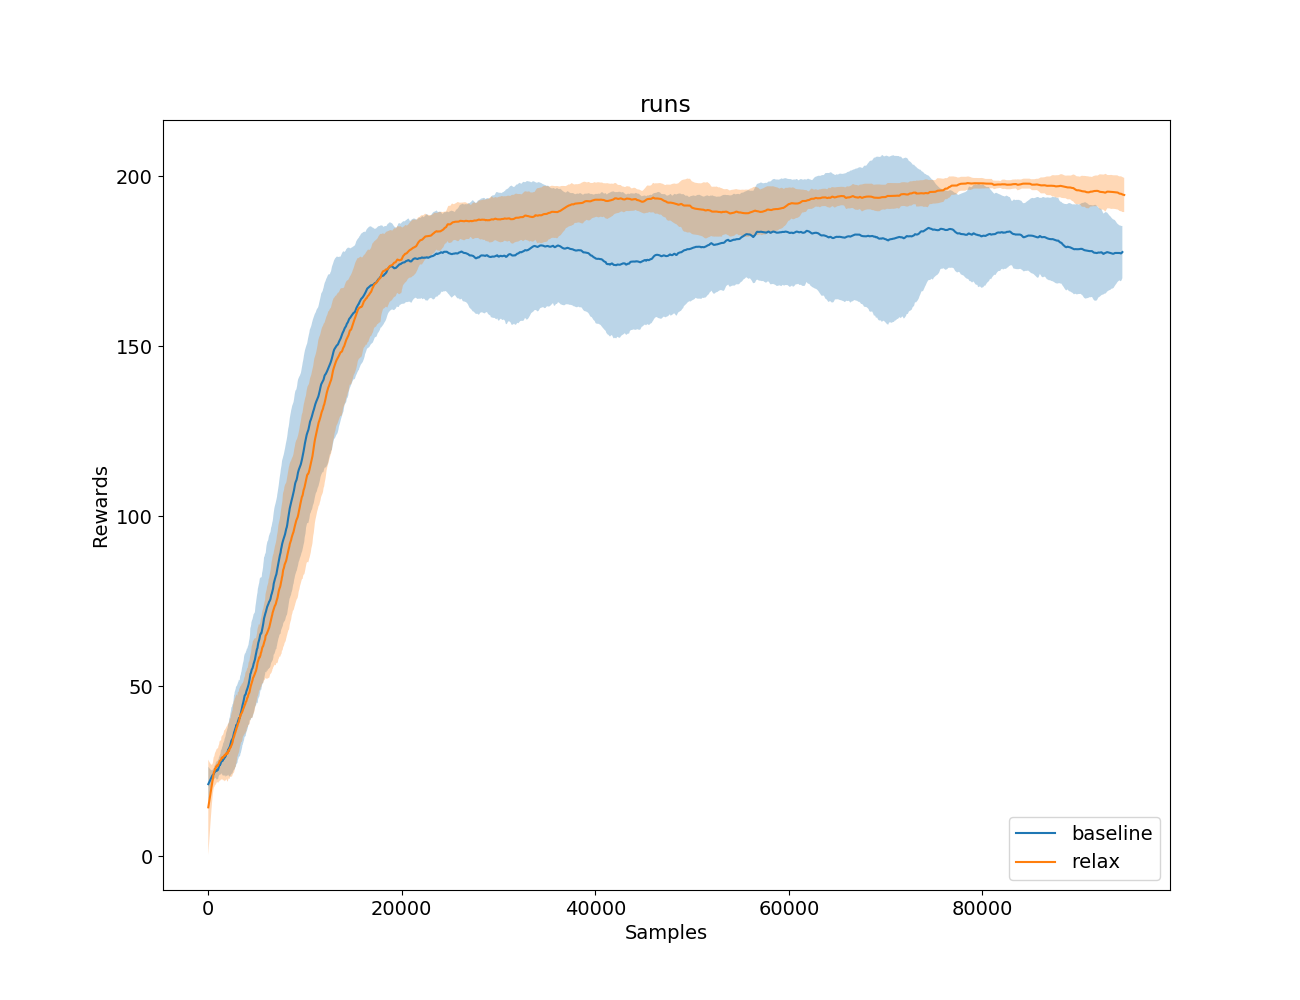
\includegraphics[width=.4\textwidth]{figures/cartpole_rewards}
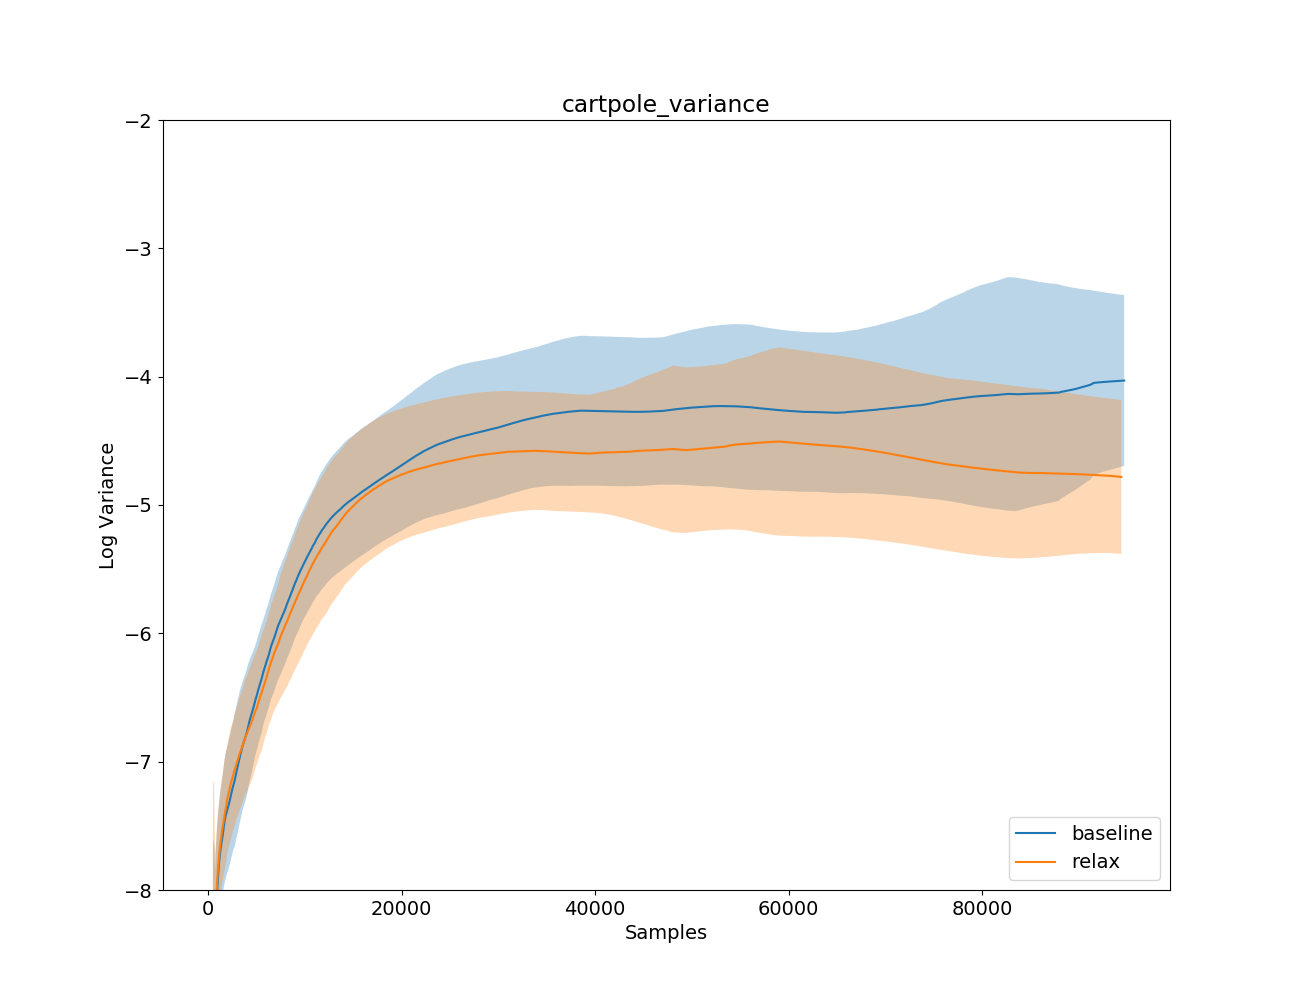
\includegraphics[width=.4\textwidth]{figures/cartpole_var}
\label{first figure}
\end{center}
\caption{Cartpole Experiments.
\emph{Left:} Rewards
\emph{Right:} Log Variances.
}
\end{figure}

\citet{mnih-dqn-2015}

[Do we use ADAM \citep{kingma2015adam} for optimization?]





\section{Related Work}
\label{related work}

\citet{miller2017reducing} further reduce the variance of reparameterization gradients in an orthogonal way.

As gradient estimators become more complex, checking their unbiasedness numerically becomes difficult.
The automatic theorem-proving-based unbiasedness checker developed by \citet{selsam2017developing} may become relevant to this line of research.

NVIL~\citep{mnih2014neural}, VIMCO~\citep{mnih2016variational}

\citet{staines2012variational} address the general problem of developing gradient estimators for deterministic black-box functions or discrete optimization.
They introduce a sampling distribution, and optimize an objective similar to ours. 

\citet{wierstra2014natural} also introduce a sampling distribution to build a gradient estimator, and consider optimizing the sampling distribution.

\citet{asadi2017mean} reduce the variance of actor-critic gradient estimates by simply summing over all possible actions.

\citet{salimans2017evolution} estimate gradients using a form of finite differences, evaluating hundreds of different parameter values in pararallel to construct a gradient estimator.
In contrast, our method is a simple-sample estimator.

\par{Generalized Reparameterization Gradients}
REBAR and the generalization in this paper uses a mixture of score function and reparameterization gradients.
A recent paper by \cite{ruiz2016generalized} unifies these two gradient estimators as the generalized reparameterization gradient (GRG).
This framework can help disentangle the various components of generalized REBAR.

REBAR innovation as further decomposition the correction term into secondary reparameterization components
note this is a recursive application of the principles of GRG
observe that the GRG suggests this recursive application to components of an estimator
propose that other estimators could be similarly recursively decomposed?




\section{Conclusions and Future Work}
\label{conclusion}

Other possible applications:

GANs \citep{goodfellow2014generative} that generate text or other discrete objects.

Learning to parse \citep{kusner2017grammar}

VAEs with continuous latent variables but non-differentiable likelihood functions.


%\section*{Acknowledgements}  % Uncomment for arxiv
%We thank Tian Qi Chen for helpful discussions.

\bibliography{bibliography}
\bibliographystyle{iclr2018_conference}




\section{Appendix A: Control Variates}
% basic definitions following level of detail in Tucker 2017


% ** Questions to answer: 
% (1) is z-tilde a clever way of using Rao-Blackwellization for a part of the reparameterization gradient? This would mean that the reparameterization z-tilde is related to the sufficient statistic of the estimator...
% (1) also maybe: the Q function has the opportunity to learn an estimator based on the sufficient statistics of the model, which by Rao-Blackwell-Kolmogorov is lower variance
% (2) What's a better notation to keep the dependence of z on $\theta$ in view?
% (3) is the REBAR control variate really using the reparameterization gradient in a meaningful way? Or, is it best viewed as just another f + control variate where control variate is cleverly designed with lower variance? 


\par{Generalizing the reparameterization trick}

Write sample from distribution $s(\epsilon)$ as $\epsilon = \mathcal{T}^{-1}(\mathbf{z}; \mathbf{\nu})$ for some invertible transform $\mathcal{T}$ with variational parameters $\nu$.
write out transformed density
example: normal with standard normal $s$
example: inverse CDF of Gaussian with uniform $s$
write out expected gradient under transformation
show decomposition of expected gradient into reparameterization and correction terms 

%\par{Applying GRG to REBAR}

%show mapping of terms
%note denser derivation in REBAR appendix

%\par{Interpreting REBAR through GRG}



\section{Appendix B: Categorical variables}

Let $G_{1:k} = -\log-\log(U_{i:k})$ be samples from the Gumbel distribution, and learnable parameters $(\alpha_1, \dots, \alpha_k)$ be interpreted as some unnormalized parameterization of the discrete distribution under consideration.
Then, consider the following sampling procedure: for each k, find the k that maximizes $\log \alpha_k - G_k$, and then set $D_k=1$ and $D_{i \neq k} = 0$. The Gumbel-Max trick states that sampling from the discrete distribution is equivalent to taking this argmax, that is, $p(D_k = 1) = \alpha_k / \sum_{i=1}^n \alpha_i$.

Since taking an argmax is still a discontinuous operation, \cite{maddison2016concrete} and \cite{jang2016categorical} proposed further relaxing the argmax operator through the softmax function with an additional temperature parameter $\lambda$:
\begin{equation}
x_k = \frac{\exp\{( \log \alpha_k+ G_k) / \lambda\}}{\sum_{i=1}^n\exp\{( \log \alpha_i+ G_i) / \lambda\}}
\end{equation}
This relaxation allows values within the simplex, but in the low temperature limit, it becomes exactly the discrete argmax.
One limitation of the concrete distribution is that it is a biased estimator except in limiting temperature.
In other words, a small amount of bias is present for a non-zero temperature.

\end{document}
